\section{Object Detection (OD)}
1. Predict bbox labels and confidence. \\ 
\textbf{Localization:} Sliding win.  \\
\textbf{Classification:} Often SVM.

\subsection{Eval Metrics}
\[
   \text{IoU} = \frac{\text{intersection}}{\text{union}}
   \] 
\[
   \text{Precision} = \frac{\text{TP}}{\text{TP} + \text{FP}}
   \] 
\[
   \text{Recall} = \frac{\text{TP}}{\text{TP} + \text{FN}}
   \]  \\
4. \textbf{mAP:} Mean AP over all classes.

\subsection{Sliding Window-Based OD}
1. Sliding windows over multi scales/sizes.  \\
2. \textbf{Challenges:} Inefficient for large-scale datasets.  \\
3. \textbf{Human Detection w/ HOG:}  
   a. Train pedestrian template w/ SVM.  \\
   b. Apply template across img.  \\
   c. Use local maxima of response for detection.  \\
   d. Multi-scale detection w/ HOG pyramid.

\subsection{Discriminative Part-Based Models (DPM)}
1. Objects are decomposed into parts.  \\
2. Example: Deformable Part-based Models (DPM).  \\
   a. Detect parts and combine using an ensemble.  \\
   b. 'Springs': spatial connections between parts.\\

\subsection{Proposal-Based OD}
1. \textbf{Selective Search:}  
   Uses diverse cues to merge superpixels into regions for better bbox proposals.  \\
2. \textbf{EdgeBoxes:}  
   a. Exploits edge info w/ a trained edge detector.  
   b. Forms object-like groupings (objects tend to be enclosed by edges).

\subsubsection{R-CNN (Region-Based CNN)}
1. Region proposals + CNN features.  
2. \textbf{Pipeline:}  
   a. Regions generated using Selective Search.  \\
   b. Features extracted w/ AlexNet.  \\
   c. Final detector: Non-max suppression (NMS) + linear SVM.  \\
   d. Bbox regression refines proposals.  \\
3. \textbf{Pros:} High detection accuracy.  \\
4. \textbf{Cons:}  
   a. Not end-to-end trainable.  \\
   b. Multistage pipeline makes train/eval slow.

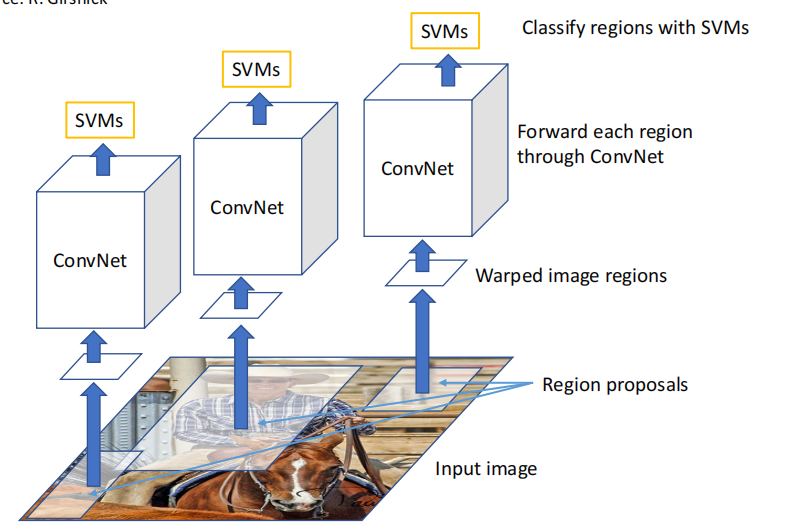
\includegraphics[width=1\linewidth]{images/rcnn.png}

\subsubsection{Fast R-CNN}
1. Uses shared feature map from CNN.  \\
   a. In R-CNN, a separate CNN is trained for each proposal.  \\
   b. Fast R-CNN fixes this by using a single shared feature map.  \\
2. \textbf{ROI Pooling:} 
   Region proposals are mapped to the shared feature map. Regions are resized to the same size through ROI pooling. \\
3. Two losses:   \\
   a. Softmax loss for classification.   \\
   b. Bbox regression loss. \\

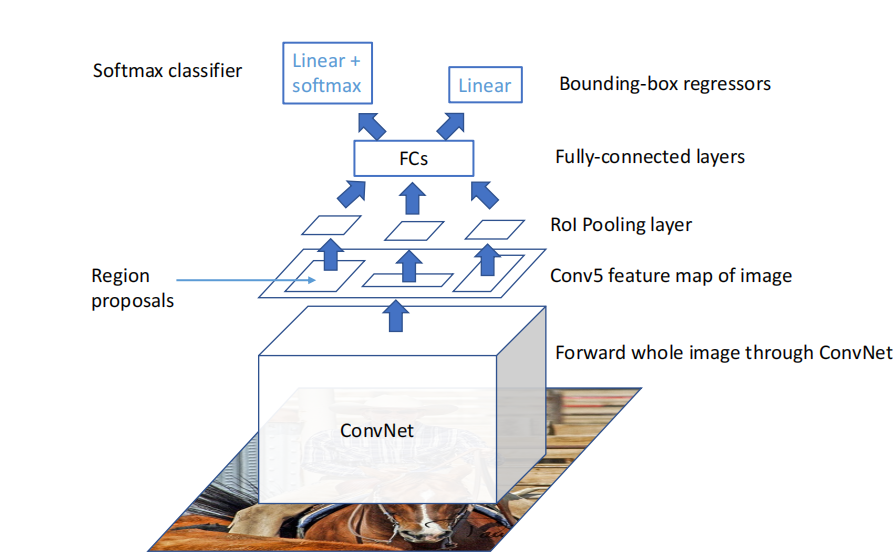
\includegraphics[width=1\linewidth]{images/fast-rcnn.png}

\subsubsection{Faster R-CNN}
1. Adds a Region Proposal Network (RPN) to the pipeline. \\
2. \textbf{Key Components:} \\
   a. Fully conv net: \\
      i. Input: Shared feature map. \\
      ii. Output: Region proposals. \\
   b. Fixed-size window over conv layers. \\
      i. Predict obj / no obj for proposals. \\
      ii. Regress bbox coords w.r.t. anchors. \\
3. 2 classification loss and 2 bbox regression loss. \\

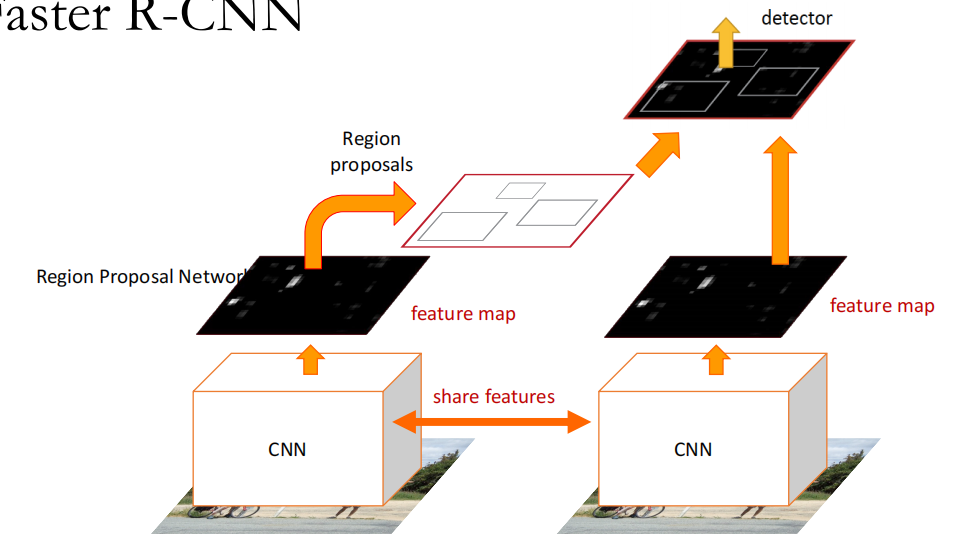
\includegraphics[width=0.9\linewidth]{images/faster-rcnn.png}

\subsubsection{YOLO (You Only Look Once)}
1. Combines classification and regression. \\
2. \textbf{Pipeline:} \\
   a. Image divided into $S \times S$ grids. \\
   b. For each grid, predict: \\
      i. Bboxes. \\
      ii. Confidence scores. \\
      iii. Class probs. \\
   c. Box filtering w/ NMS. \\
3. \textbf{Pros:} \\
   a. Real-time detection. \\
   b. Captures global context. \\
   c. Simple design. \\
4. 3 Losses: Localization loss, confidence loss, classification loss. \\
